We perform extensive experiments on randomly generated maps and analyze the results to evaluate the performance of Nav A3C on navigation.
%% Experiments
% Introduce the Deep-RL method we use. Based on earlier work.
% Describe the differing environments we are trying the method on. It is important that the reader understands how environment complexity increases over time. In order of increasing difficulty we have:
% Static spawn, static goal, static maze 
% - deterministic, easy, memorizable
% 
% 
% Random spawn, static goal, static maze 
% - Agent must recognize a path upon revisiting it
% - Must memorize multiple paths to goal
% 
% 
% Static spawn, random goal, static maze 
% - Maze environment needs to be learned in some sense
% - Agent needs to remember the maze to navigate to the goal repeatedly
% 
% 
% Random spawn, random goal, static maze
% - agent needs to dynamically remember the maze and goal location
% - can it first find the goal and then repeatedly traverse to it in shorter amounts of time?
% Random spawn, random goal, random maps
% - can the agent learn a generalized navigation strategy that performs implicit mapping
% - If it can’t what is it actually learning?
% Effect of variations: An agent that was trained on planar environments will fail to generalize but does an agent trained on variations environment generalize to planar environments.
% How do learned navigation strategies extend to unknown environments? Is there every any aspect of path planning? 


\subsection{Replicating Learning to navigate}
Since \cite{MiPaViICLR2017} did not release their source code, so we implemented their pipeline by starting a fork from \texttt{universe-start-agent}\cite{OpenAI2017UniverseStarterAgent}.

To make sure that we replicate \cite{MiPaViICLR2017} results, we setup the experiment as similar to what was described in the paper. We use the same game environment Deepmind Lab \cite{BeLeTeARXIV2016} as used by \cite{MiPaViICLR2017}. But there are few differences that are note worthy
\begin{itemize}
\item But unlike, \cite{MiPaViICLR2017} instead of hand picking the maps to run experiments on, we chose to run the experiments on randomly generated maps.
We create a set of randomly generated maps by a textbook depth first search based algorithm with randomly introduced loops. The 
\item We use a smaller action space than \cite{MiPaViICLR2017}. We use an action space of four actions move forward, move backward, rotate left and roate right, while \cite{MiPaViICLR2017} use an action space of 8 actions ``the agent can rotate in small increments, accelerate forward or backward or
sideways, or induce rotational acceleration while moving.''
\item We use randomly colored walls for robustness against textures.
\item We use wall penality to make sure that the agent does not run into walls too often.
\item All our maps have ``thick'' walls which means that each wall thickness is same as thickness of the corridor, while maps in \cite{MiPaViICLR2017}
\end{itemize}

Next, we evaluate the algorithm on increasing order of difficulty as described in Section~\ref{sec:navtasks}. The results of our experiments are shown in Fig~\ref{fig:latency-goal-reward}.
We evaluate the Nav-A3C\cite{MiPaViICLR2017} algorithm on randomly chosen ten maps with increasing difficulty.
We change the randomness of either the spawn point or the goal location.
We note that the increasing randomness gradually reduce the maximum reward achived and the number of times the goal is reached. As expected, the variance in reward and number of times goals is reached also increases with randomless.

\subsection{Evaluation Metrics}
We report three evaluation metrics in all our experiments, Reward, Average number of goal hits and \LatencyOneGtOne. We run evaluations on a map for 100 episodes and take the mean and standard deviation of the rewards per episode and number of goal hits per episode. Even though reward includes rewards due to apples and negative rewards due to wall penalities, the reward due to goal dominates dominates the reward metric making reward approximately ten times the average goal hits.

The \LatencyOneGtOne is defined as the ratio of time take to find the goal first time to the average time take to find goal thereafter.
Note that whenever the goal location is ``Random'' (different in each episode but same for the episode), untill the goal is found for the first time, the agent is just exploring the map.
After the first goal hit, the agent should be able to exploit the location of the goal to find the goal in shorter times.
Hence a \LatencyOneGtOne value greater than one indicates that the algorithm is able to successfully exploit information gathered during goal finding exploration.


\begin{figure*}%
  \vspace{-4em}%
  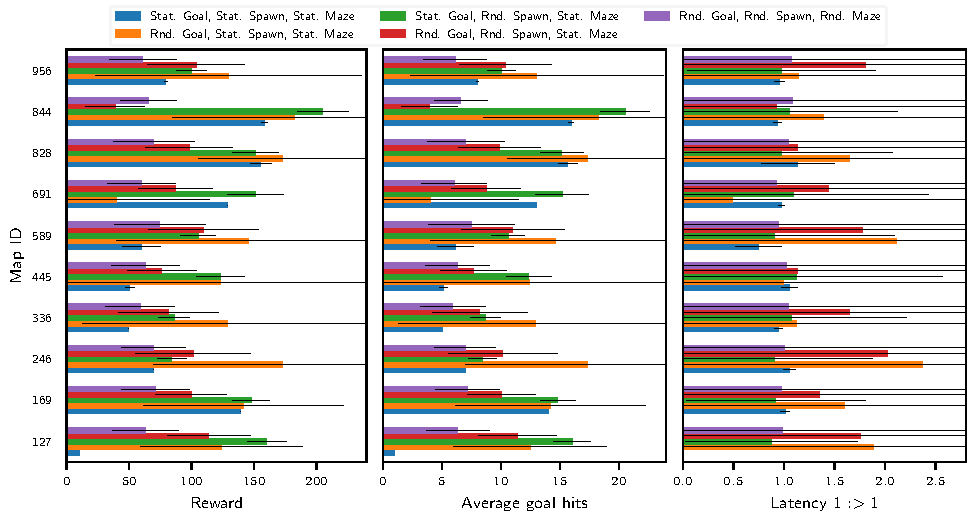
\includegraphics[width=\linewidth]{images/plot_summary_bar_plots.pdf}%
  \vspace{-1em}%
  \caption{We evaluate the Nav-A3C\cite{MiPaViICLR2017} algorithm on randomly chosen ten maps with increasing difficulty. Vertical axes is one of the ten maps on which the agent was trained and evaluated. Horizontal axes are different evaluation metrics.
    The abbreviations in legend are as follows: ``Stat G'' stands for
    static goal location throughout the training and testing cycle.
    While ``Rand G'' stands for random goal for each episode.
    Similarly ``Stat S'',``Rand S'', ``Stat M'', ``Stat S''  stands for static spawn, random spawn, static maze and random maze respectively.
    We change the randomness of either the spawn point or the goal location. We note that when the goal is static then rewards are consitently higher as compared to random goal while static spawn location and random spawn location are roughly close to each other within bounds of uncertainity. As expected, switching each variable from static to random increases the standard deviation on the results.
    The \LatencyOneGtOne metric is only worth analyzing when the goal is random because the metric captures how well the agent exploits the additional knowledge of goal location after exploring the maze for goal in the first attempt.}%
\label{fig:latency-goal-reward}%
\end{figure*}

\begin{figure}%
  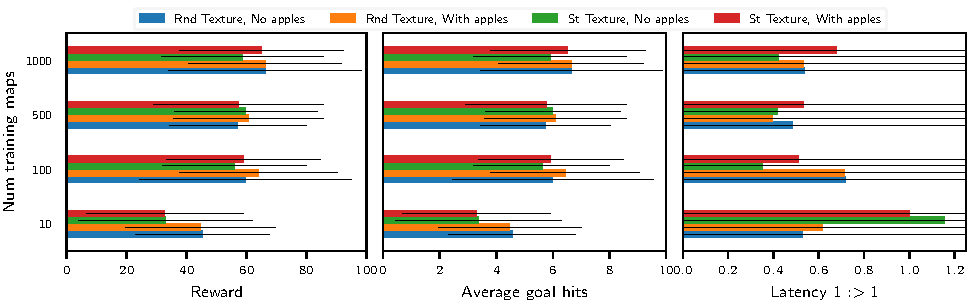
\includegraphics[width=\linewidth]{images/plot_ntrain_summary.pdf}%
  \vspace{-1em}%
  \caption{Effect of number of training maps}
  \label{fig:num-training-maps}
\end{figure}
